% -*- mode: noweb; noweb-default-code-mode: R-mode; -*-
\documentclass[a4paper]{article}
\usepackage[margin=0.5in]{geometry}
\usepackage{/Library/Frameworks/R.framework/Resources/share/texmf/Sweave}


\title{R Code for Modelling Gasification and Related Processes}
\author{Bear Kaufmann\\
\normalsize{All Power Labs}\\
\normalsize{1010 Murray St., Berkeley, CA}\\
\normalsize{bear@allpowerlabs.org}
}

\begin{document}
\maketitle
\vfill
\begin{center}
\includegraphics[width=1in]{documentation/images/cc_by_sa.png}\\
This document and associated code is released as Creative Commons Attribution - Share Alike.
For more information on this license, please visit http://creativecommons.org/about/licenses/
\end{center}
\newpage
\section{Description}
\paragraph{
	The code here is used to help in modelling gasification reactions and related processes.
}
\paragraph{
This document is an early stage exploration of models, graphics, and equations related to biomass energy. Proper citations may not be included in this text, but are generally available in the included code and data. Additional relevant publicly available data and data sets are welcomed.
}
\section{Graphs}
\subsection{Gasification Gas Composition vs. Lambda}
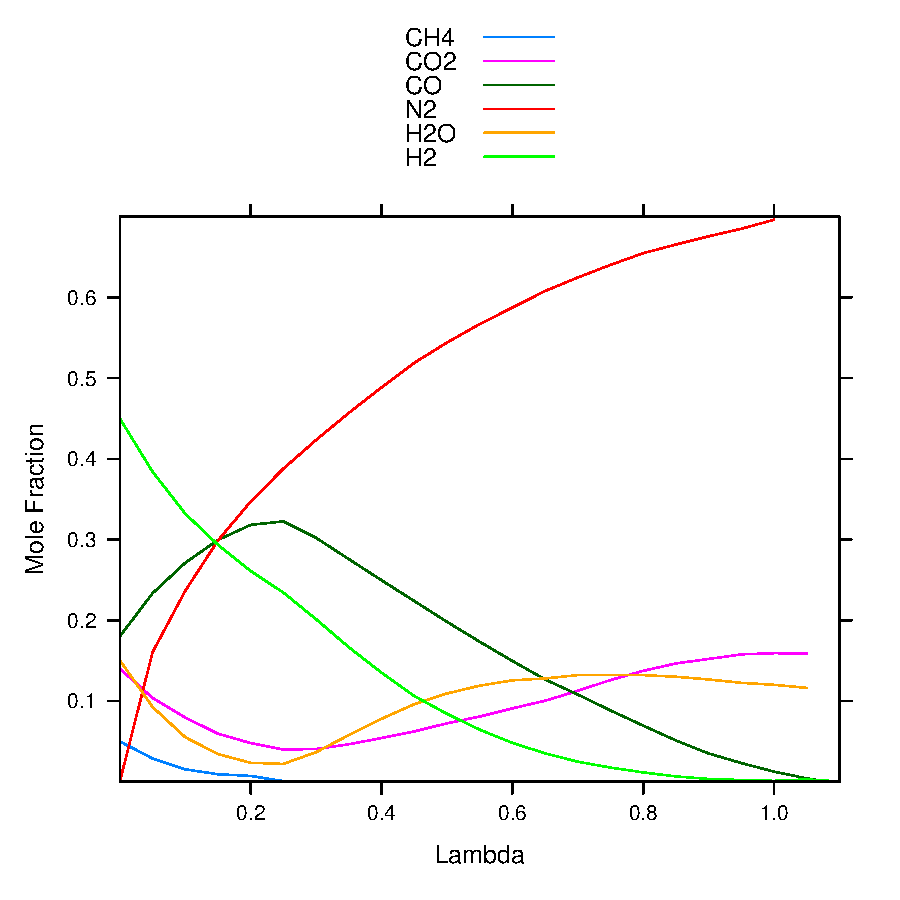
\includegraphics{documentation/images/img-001}
\\
Data from Kaupp [citation needed]
\\
\section{Van Krevelen Diagram}
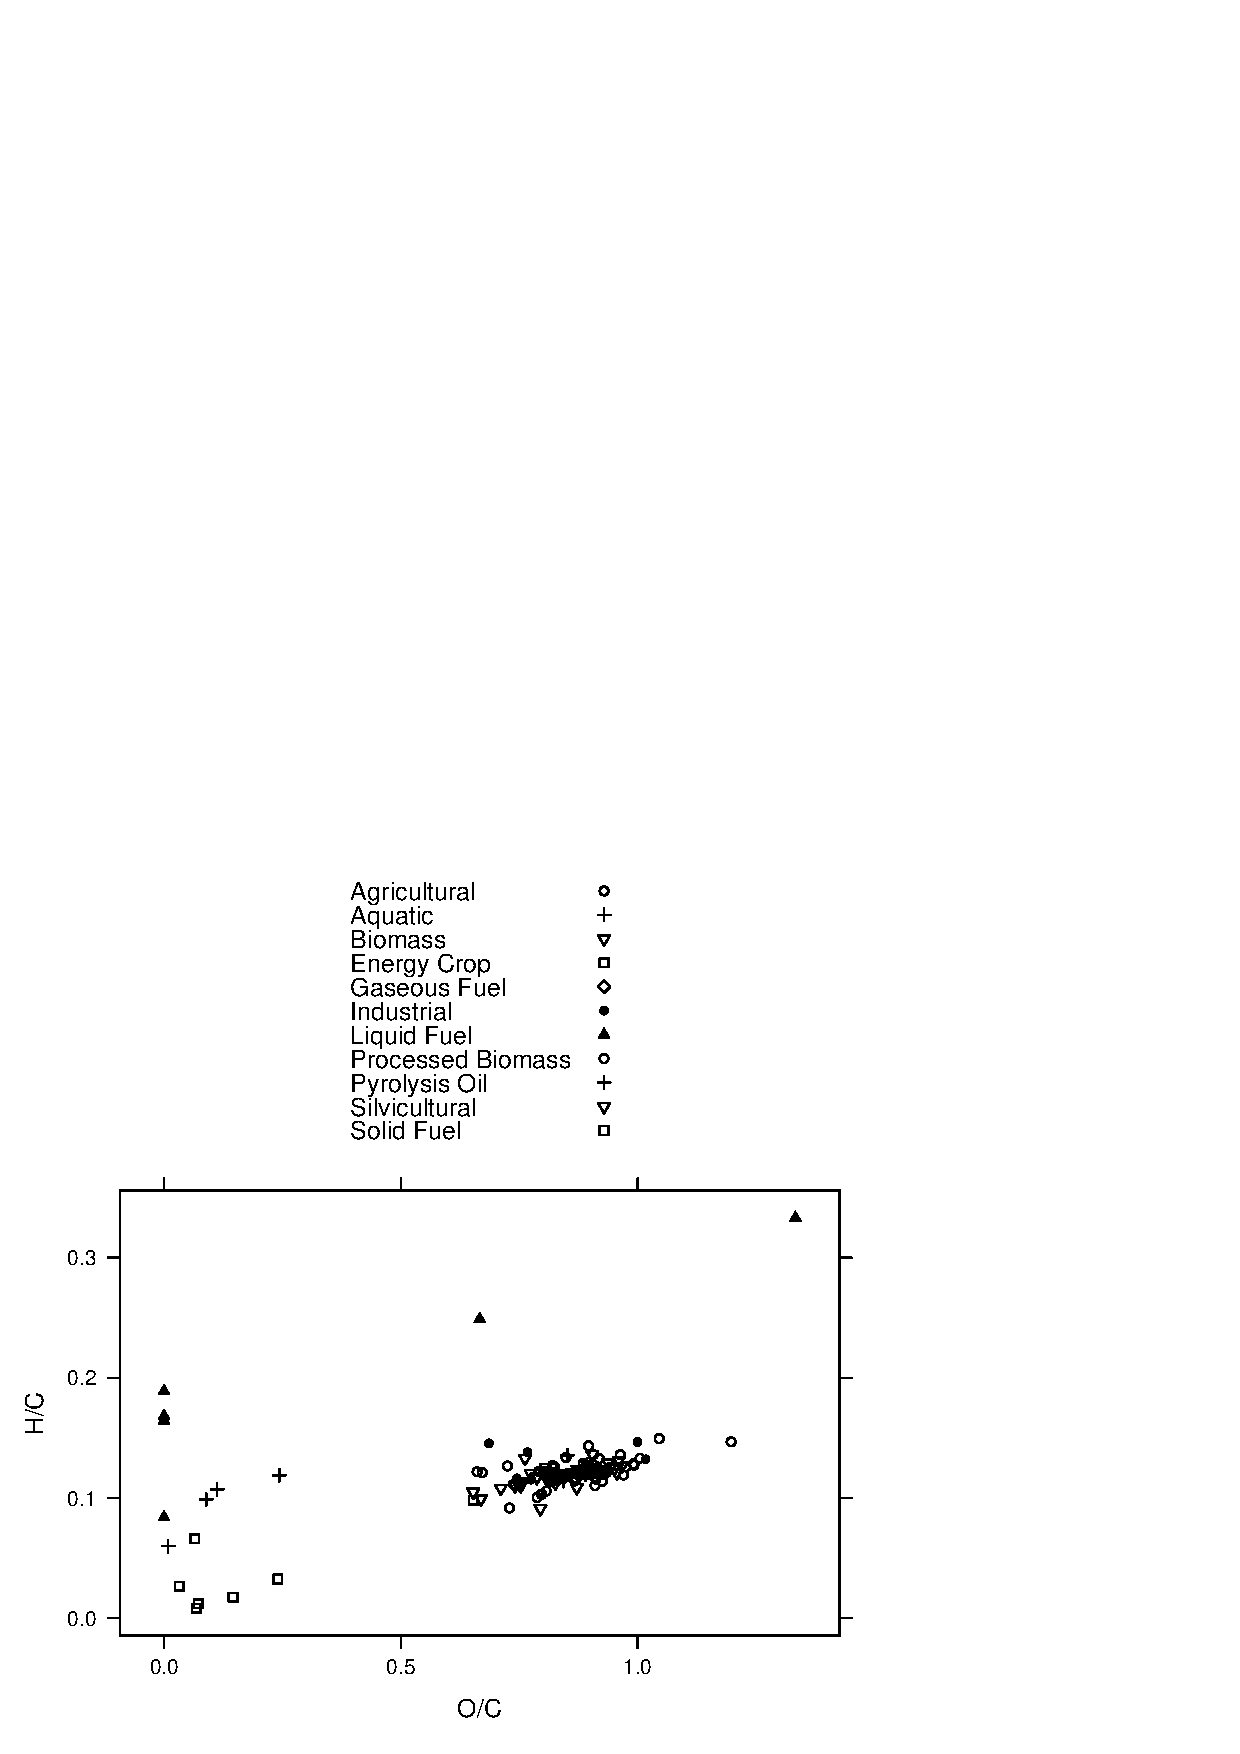
\includegraphics{documentation/images/img-002}
\\
\section{Biomass Ternary Diagram}
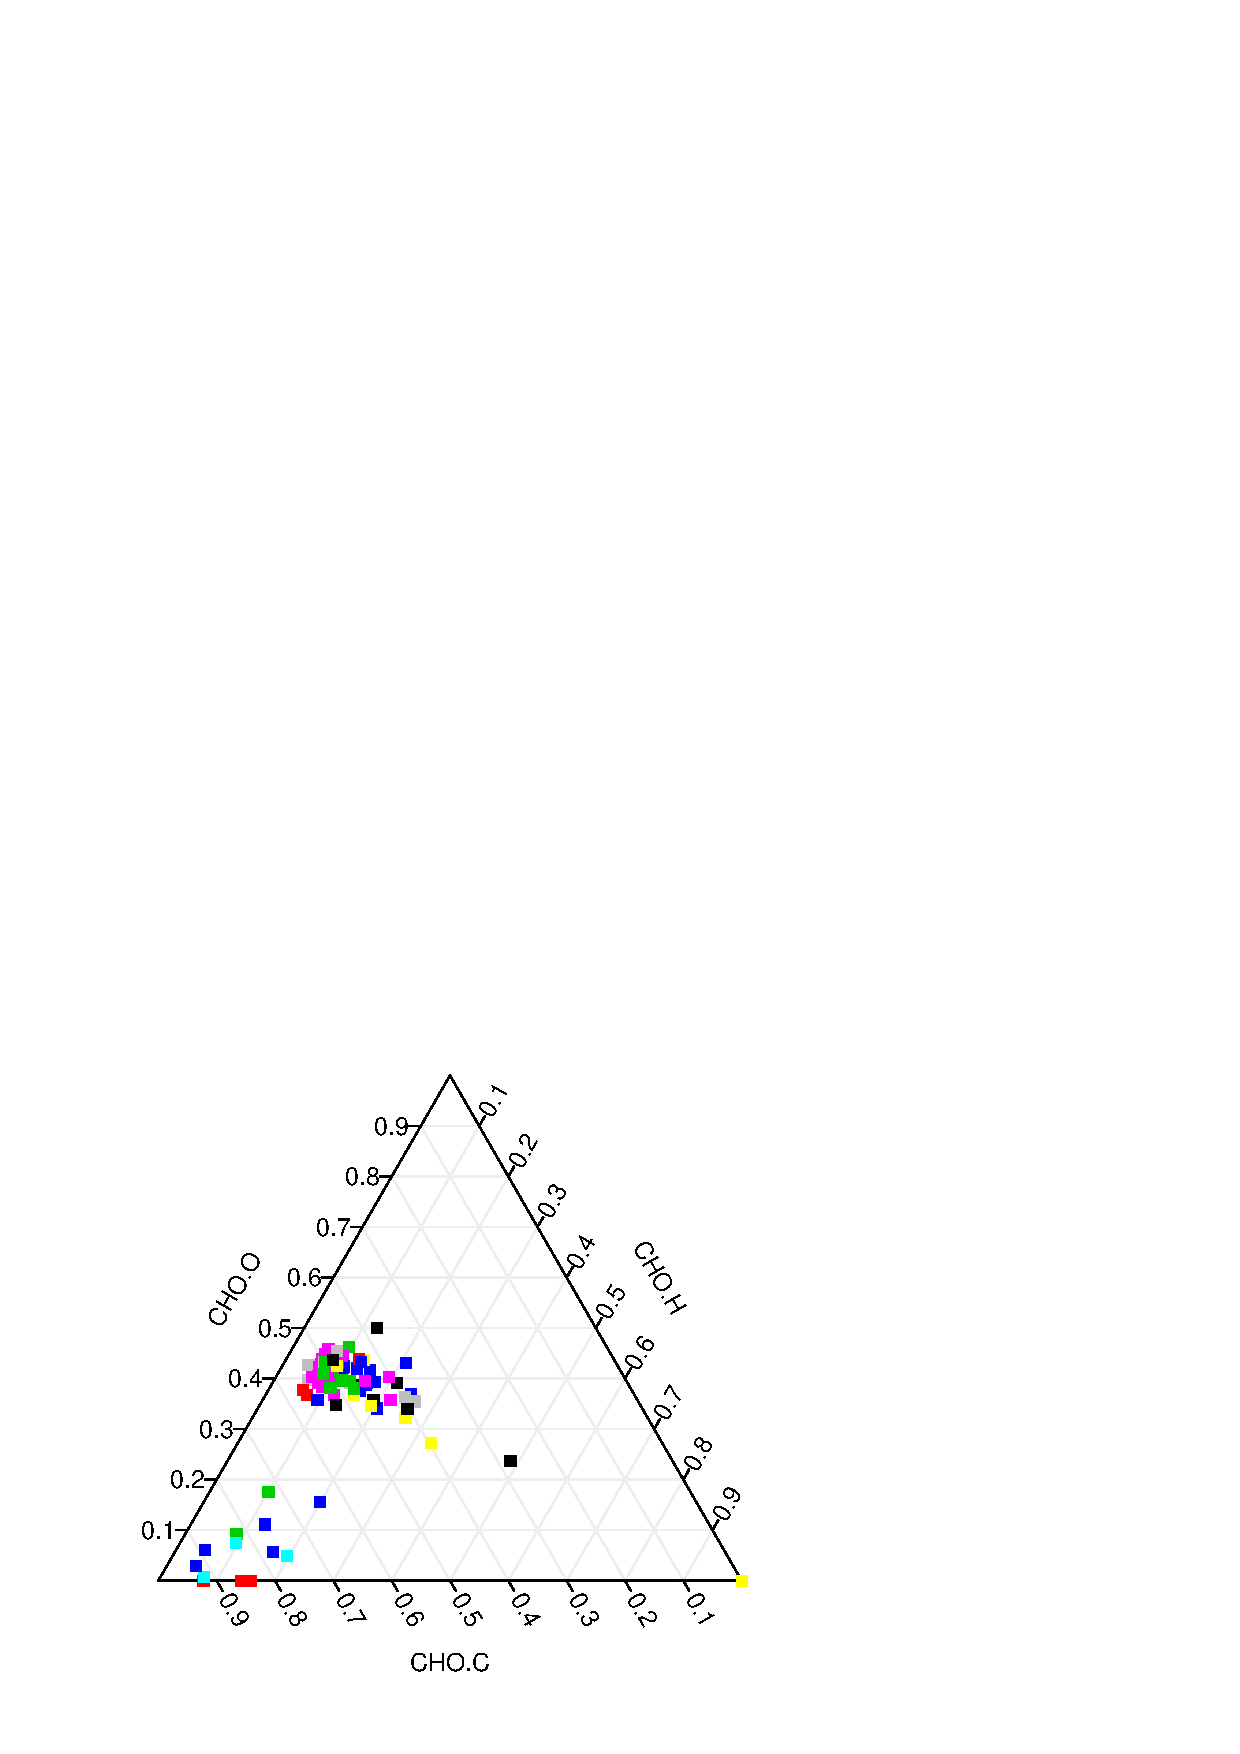
\includegraphics{documentation/images/img-003}
\\
\newpage
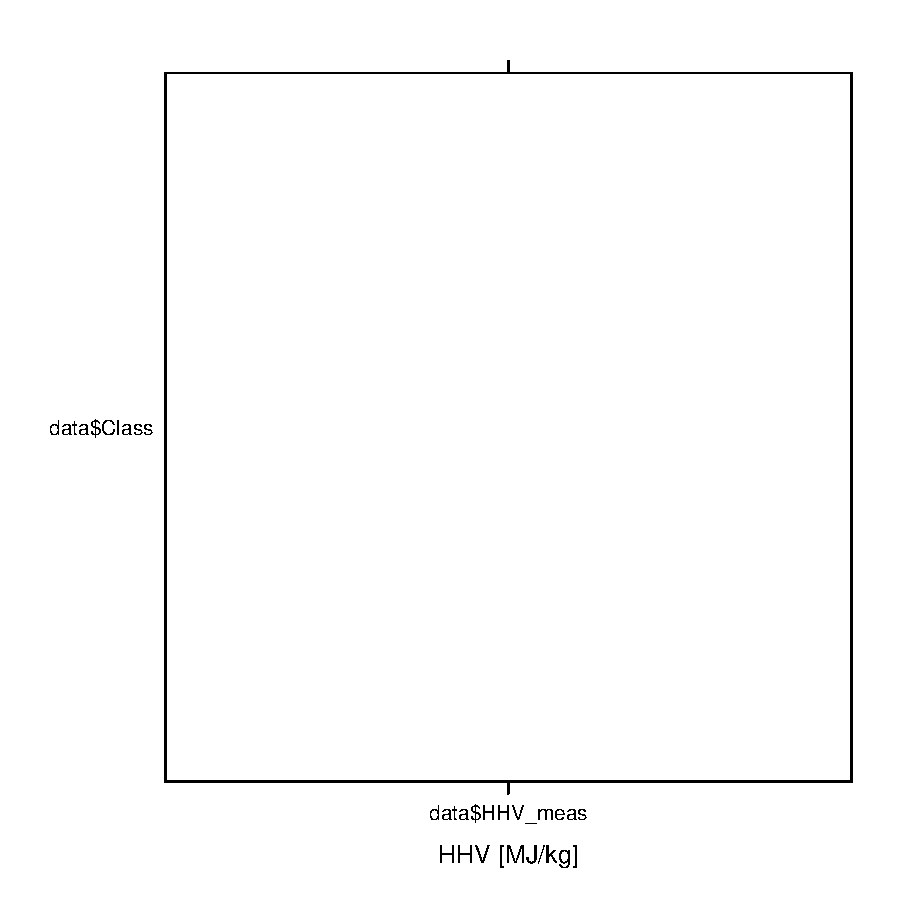
\includegraphics{documentation/images/img-004}
\\
\newpage
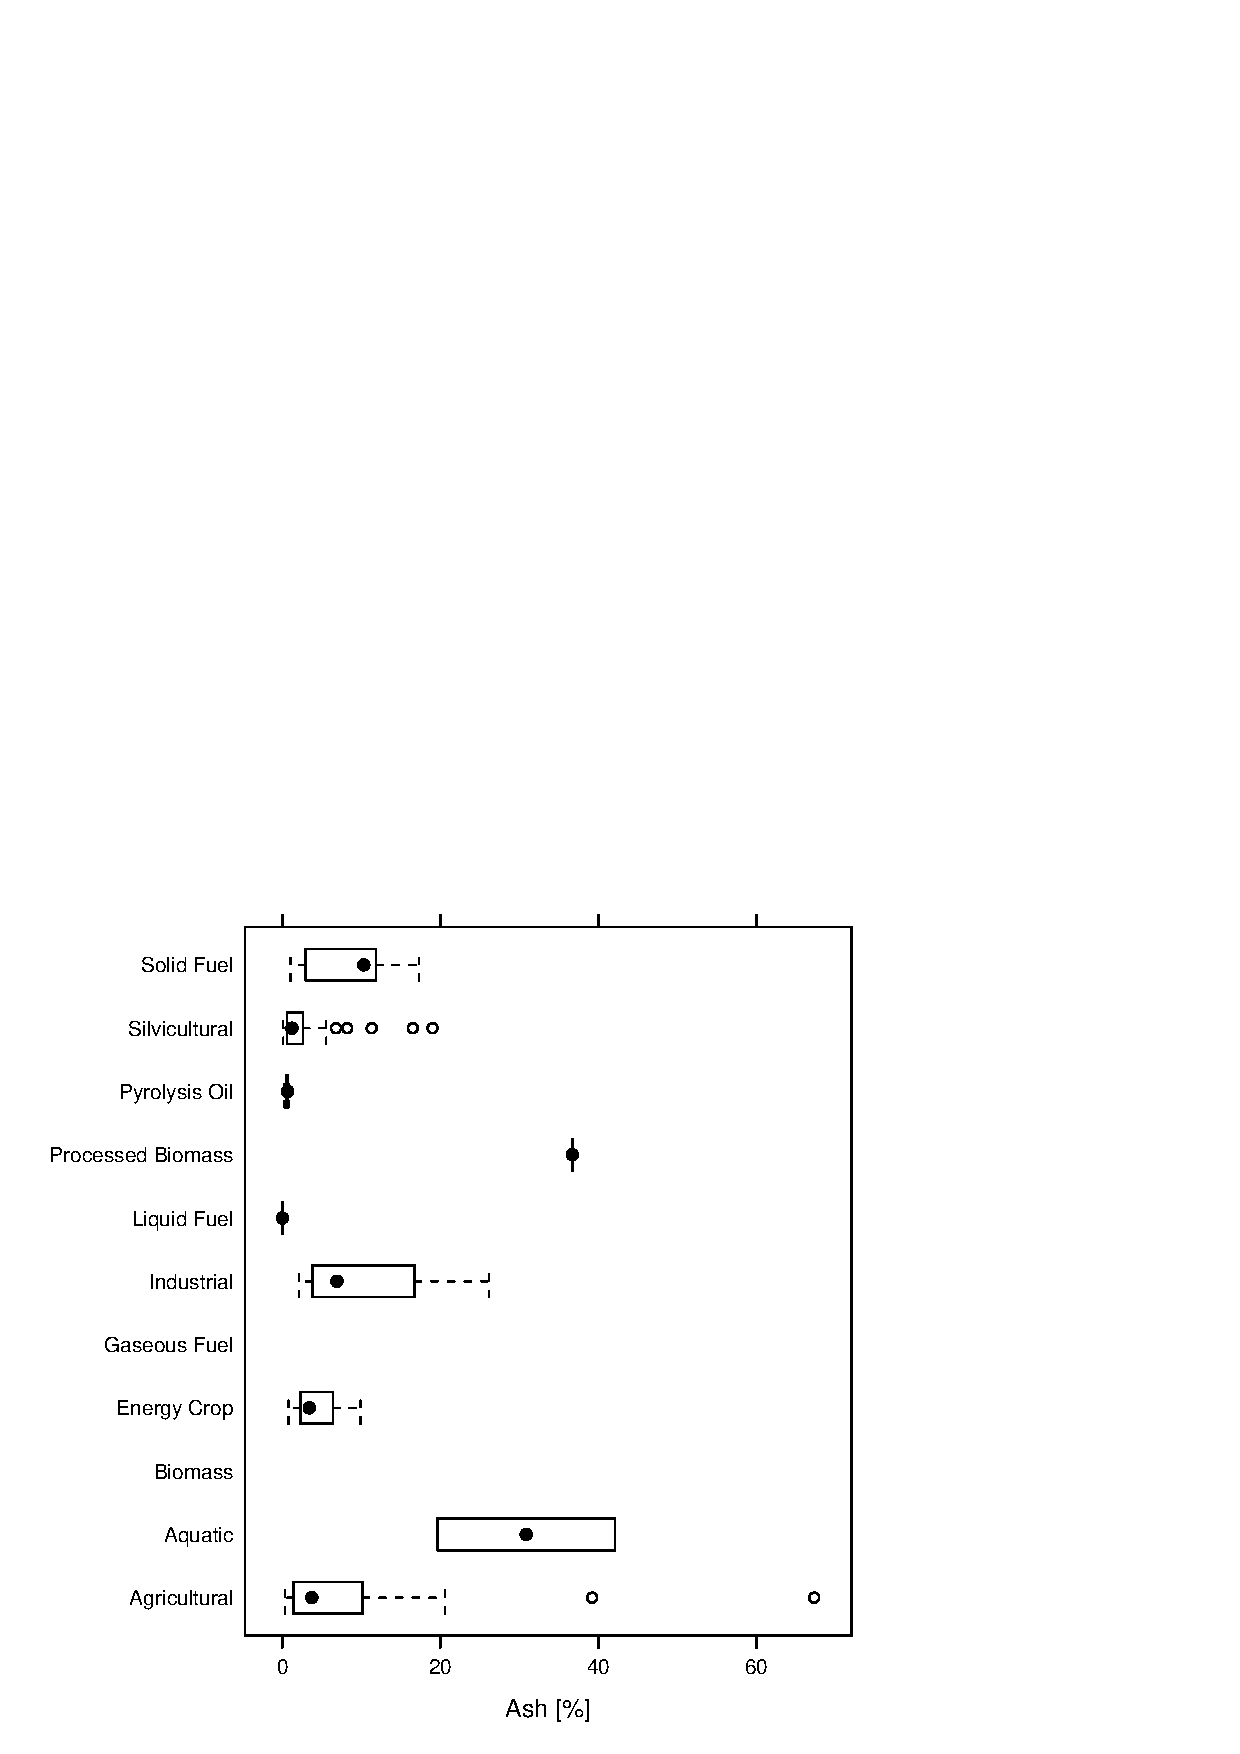
\includegraphics{documentation/images/img-005}
\\
\newpage
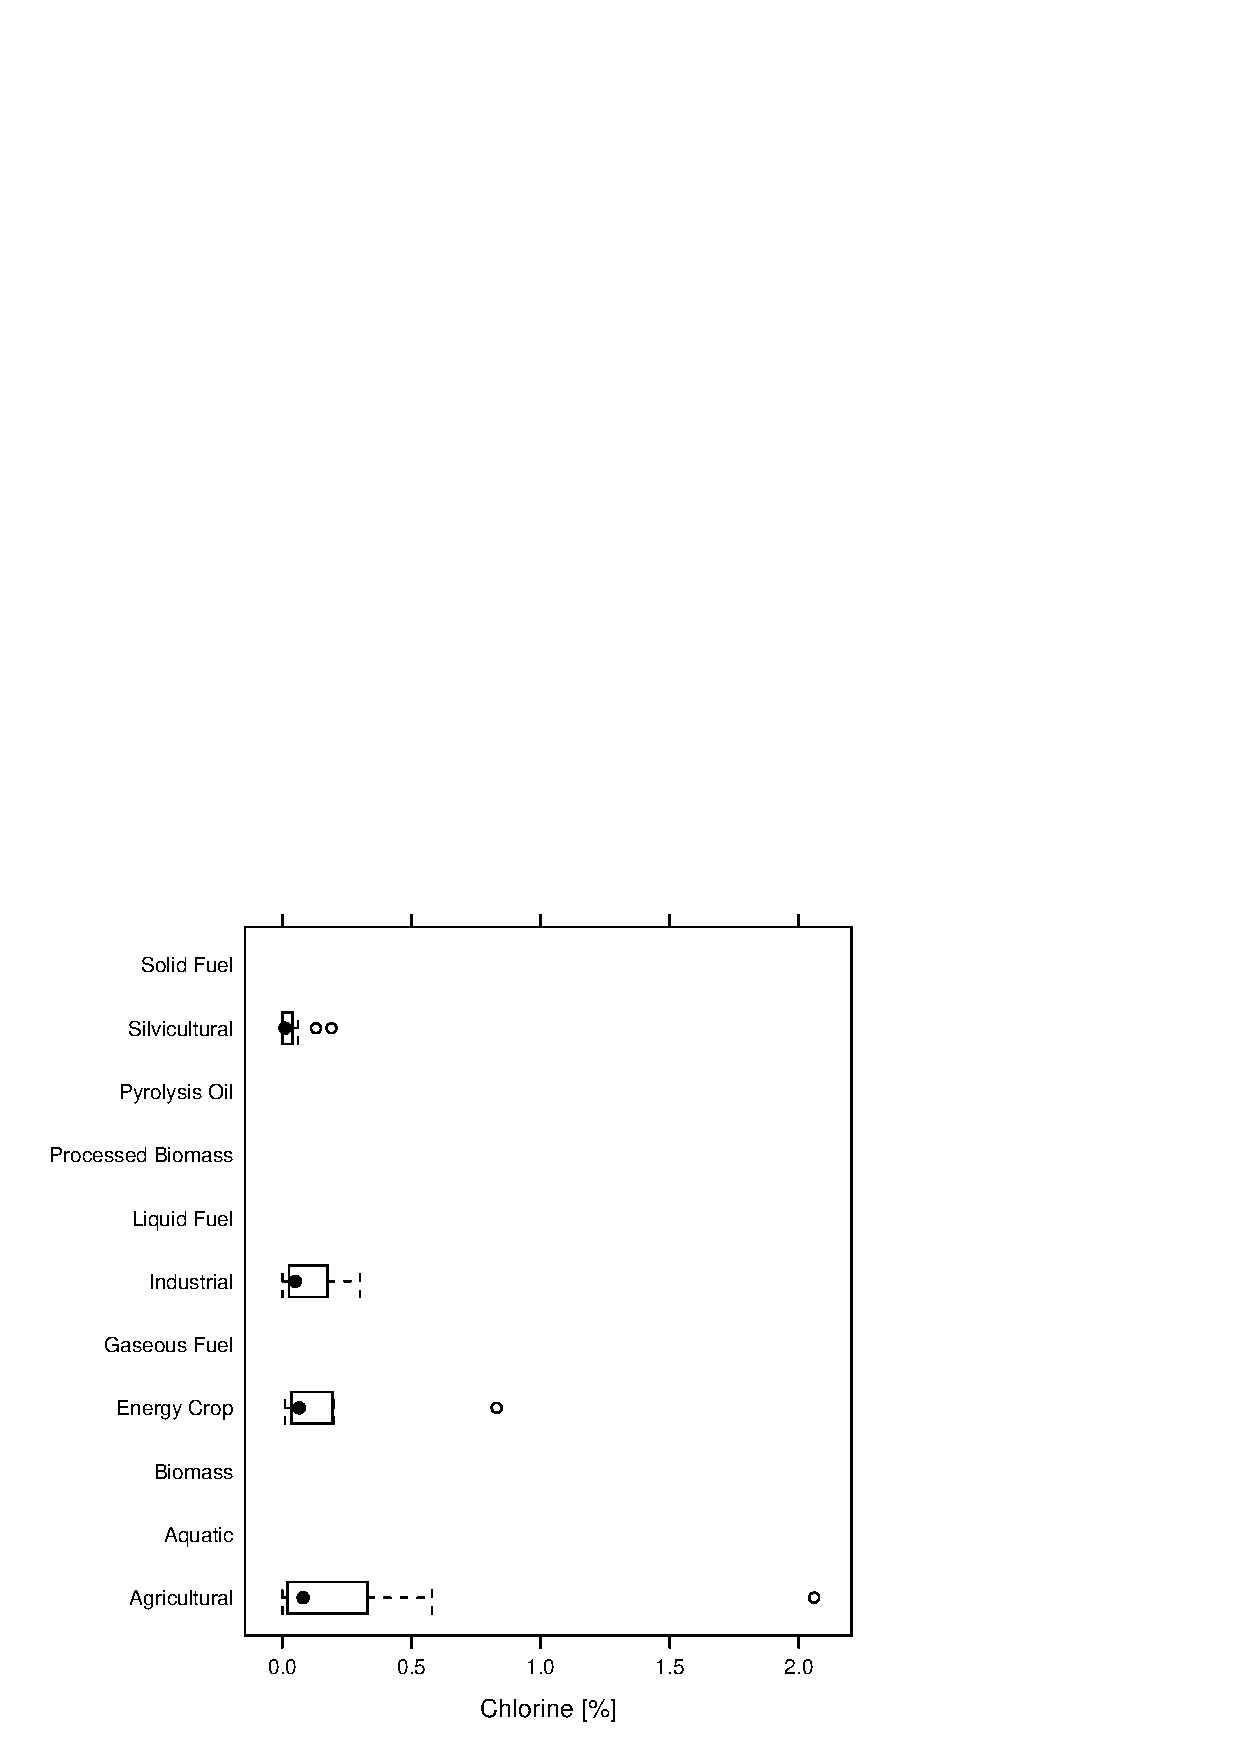
\includegraphics{documentation/images/img-006}
\\
\newpage
% latex table generated in R 2.11.1 by xtable 1.5-6 package
% Mon Jan 10 21:43:03 2011
\begin{table}[ht]
\begin{center}
\begin{tabular}{rllrrrr}
  \hline
 & Material & Entity & Fixed.Carbon & Volatiles & Ash & C \\ 
  \hline
137 & Leaves & Water Hyacinth (Florida) &  & 80.40 & 19.60 & 40.30 \\ 
  138 & Leaves & Brown Kelp,Giant, Soquel Point &  & 57.90 & 42.10 & 27.80 \\ 
   \hline
\end{tabular}
\caption{Data for Aquatic Biomass}
\end{center}
\end{table}
\section{Combustion}
\includegraphics{documentation/images/img-008}
\\

\end{document}
